\section{RP13 Progressive Enhancement}
\label{sec:principle-rp13-progressive-enhancement}

Die Client-Technologien HTML und CSS haben sich über Jahre weiterentwickelt. Dies auch meistens mit dem Hintergedanken ``Progressive Enhancement'' oder Rückwärtskompatiblität. Das bedeutet, dass die Entwicklung vielfach versucht hat, Rücksicht auf die älteren Browserversionen zu nehmen.
Deutlich sieht man diese Rückwärtskompatibilität beim neuen HTML5 Standard. Neue Formularfeldtypen wie ``tel'' oder ``email''wurden eingeführt. Browser die HTML5 nicht unterstützen, wechseln bei einem für sie unbekannten Typ zum normalen Textfeld zurück.

\begin{lstlisting}[language=HTML, caption={Formularfeld mit HTML5, welches eine Telefonnummer erwartet}, label={lst:html5TelInput}]
<input type="tel" name="telefon">
\end{lstlisting}

Natürlich gibt es keine Regel ohne Ausnahme. Manche Tags, die im HTML5 Standard eingeführt wurden, werden überhaupt nicht beachtet. Dies kann vor allem bei Versionen ``kleiner als Neun'' des Internet Explorers beobachtet werden.

\subsection*{Geplante Umsetzung}
Die Beispielanwendung soll, wie bereits in Kapitel \ref{sec:requirments-engineering-nonfunctionals} erwähnt, folgende Versionen unterstützen: Internet Explorer 8 und höher, Chrome 25 und höher, Firefox 19 und höher und Safari 6 und höher.

Auch Browser auf Smartphones sollten nicht vernachlässigt werden. Hierfür sollen Safari 6 und höher und Android Browser 4.0 und höher unterstützt werden.

\subsection*{Konkrete Umsetzung}
Da nicht alle geplanten und zu unterstützenden Browser HTML5 interpretieren können, musste ein kleiner Trick angewendet werden, um so die Rückwärtskompatibilität zu erhöhen. Dieser Trick heisst ``modernizr'' \cite{modernizr}, eine JavaScript-Bibliothek, welche gezielt den verwendeten Browser auf seinen Funktions- und Unterstützungsumfang von HTML und CSS überprüft. Das Resultat wird dann in einem JavaScript-Objekt gespeichert und zur Verfügung gestellt.  Zusätzlich läuft modernizr in eine kleine Schleife, um die neuen Tags (head, section, article, nav, u.w.) zu aktivieren. Das bedeutet, dass diese Tags nicht mit einem ``div''-Tag ersetzt werden müssen, wie dies sonst der Fall wäre.

Um diese Bibliothek einzubinden, hat man nichts anderes zu tun als das Skript im Header hinzuzufügen.

\begin{lstlisting}[language=HTML, caption=Einbinden von modernizr \cite{roomiesLayout}, firstnumber=11, label=lst:mdernizrLayoutServer]
<link href="/stylesheets/app.css" rel="stylesheet"/>
<script src="/javascripts/lib/custom.modernizr.js"></script>
\end{lstlisting}

Mit ``modernizr'' konnte erreicht werden, dass in allen geplanten Browser alle Elemente erscheinen, wenn auch nicht immer korrekt. Nicht immer korrekt, weil im Internet Explorer 8 die Darstellung des Bildes im oberen linken Rand nicht dem entspricht, was erwartet wurde.

\begin{figure}[H]
	\centering
	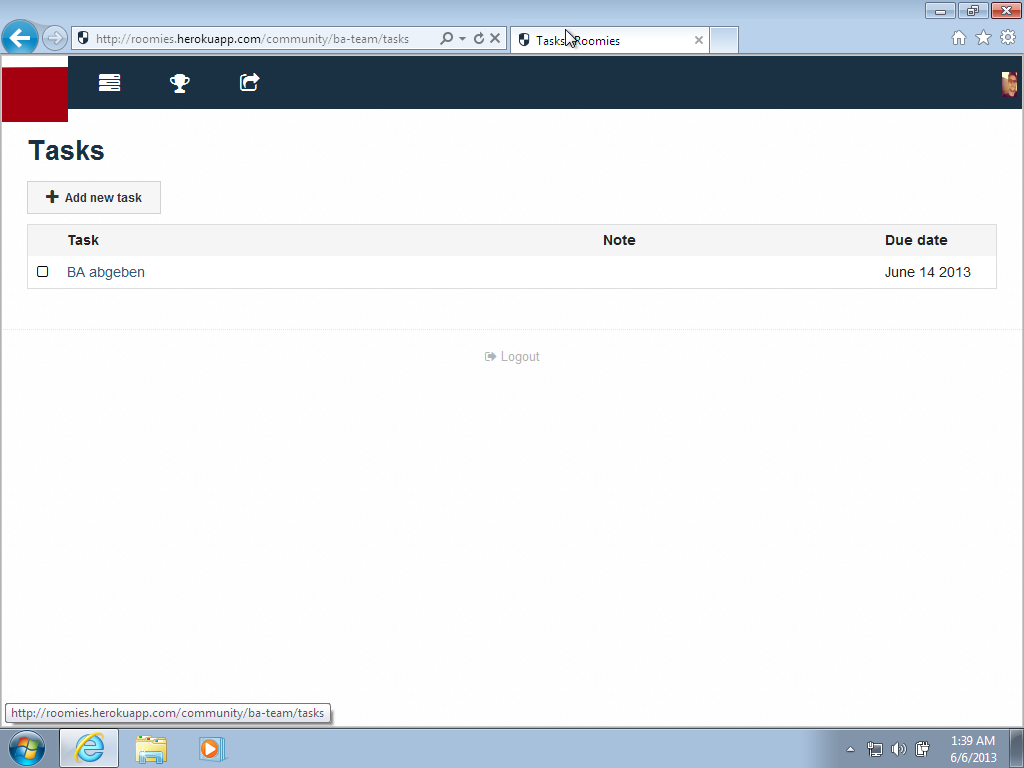
\includegraphics[width=12cm]{content/principle-demonstration/images/progressive-enhancement-ie8.png}
	\caption{Fehlerhafte Darstellung im Internet Explorer 8}
	\label{fig:iossafari-datepicker}
\end{figure}

\subsection*{Diskussion}
Je nach Zielpublikum der Webseite muss man mehr oder weniger auf die älteren Browser achten und dementsprechend eine ``Progressive Enhancement'' Technik anwenden. Mithilfe von Tools wie der erwähnten ``modernizr''-Bibliothek kann die Kompatibilität einfacher erreicht werden als ohne. Wie aber bei der Implementation auch gesehen wurde, ist es auch nicht allmächtig. Manuelles Testen ist trotzdem sehr wichtig.
\\ \\
Das Projektteam ist sich einig, dass ``Progressive Enhancement'' sehr wichtig ist. Insbesondere die Kompatibilität zu älteren Versionen von Internet Explorer stellt aber jeden Entwickler vor Probleme und verursacht immense Kosten.

Weiter ist das Projektteam der Meinung, dass diese Probleme in Zukunft zwar nicht komplett wegfallen, aber immerhin verringert werden. Microsoft hat mit Internet Explorer 10 eine ähnliche Veröffentlichungsstrategie wie die grossen anderen Browser (Firefox und Chrome) gewählt: Häufigere Veröffentlichungen in kleineren Abständen \cite{MicrosoftQuickensIEReleaseCycle}. Dies und die höhere Partizipation von Microsoft bei der Entwicklung von Standards wird in einigen Jahren den Webapplikationsentwicklern helfen, grössere Kompatiblität zwischen Browsern innerhalb von weniger Zeit zu bewerkstelligen.